\section{Hlavní stránka}

\label{nur:homepage}
Stránka používá rozvržení webu s~mapou. Podobu stránky lze vidět na obrázku \ref{fig:tur:homepage}.

\begin{figure}[!h]
    \centering
    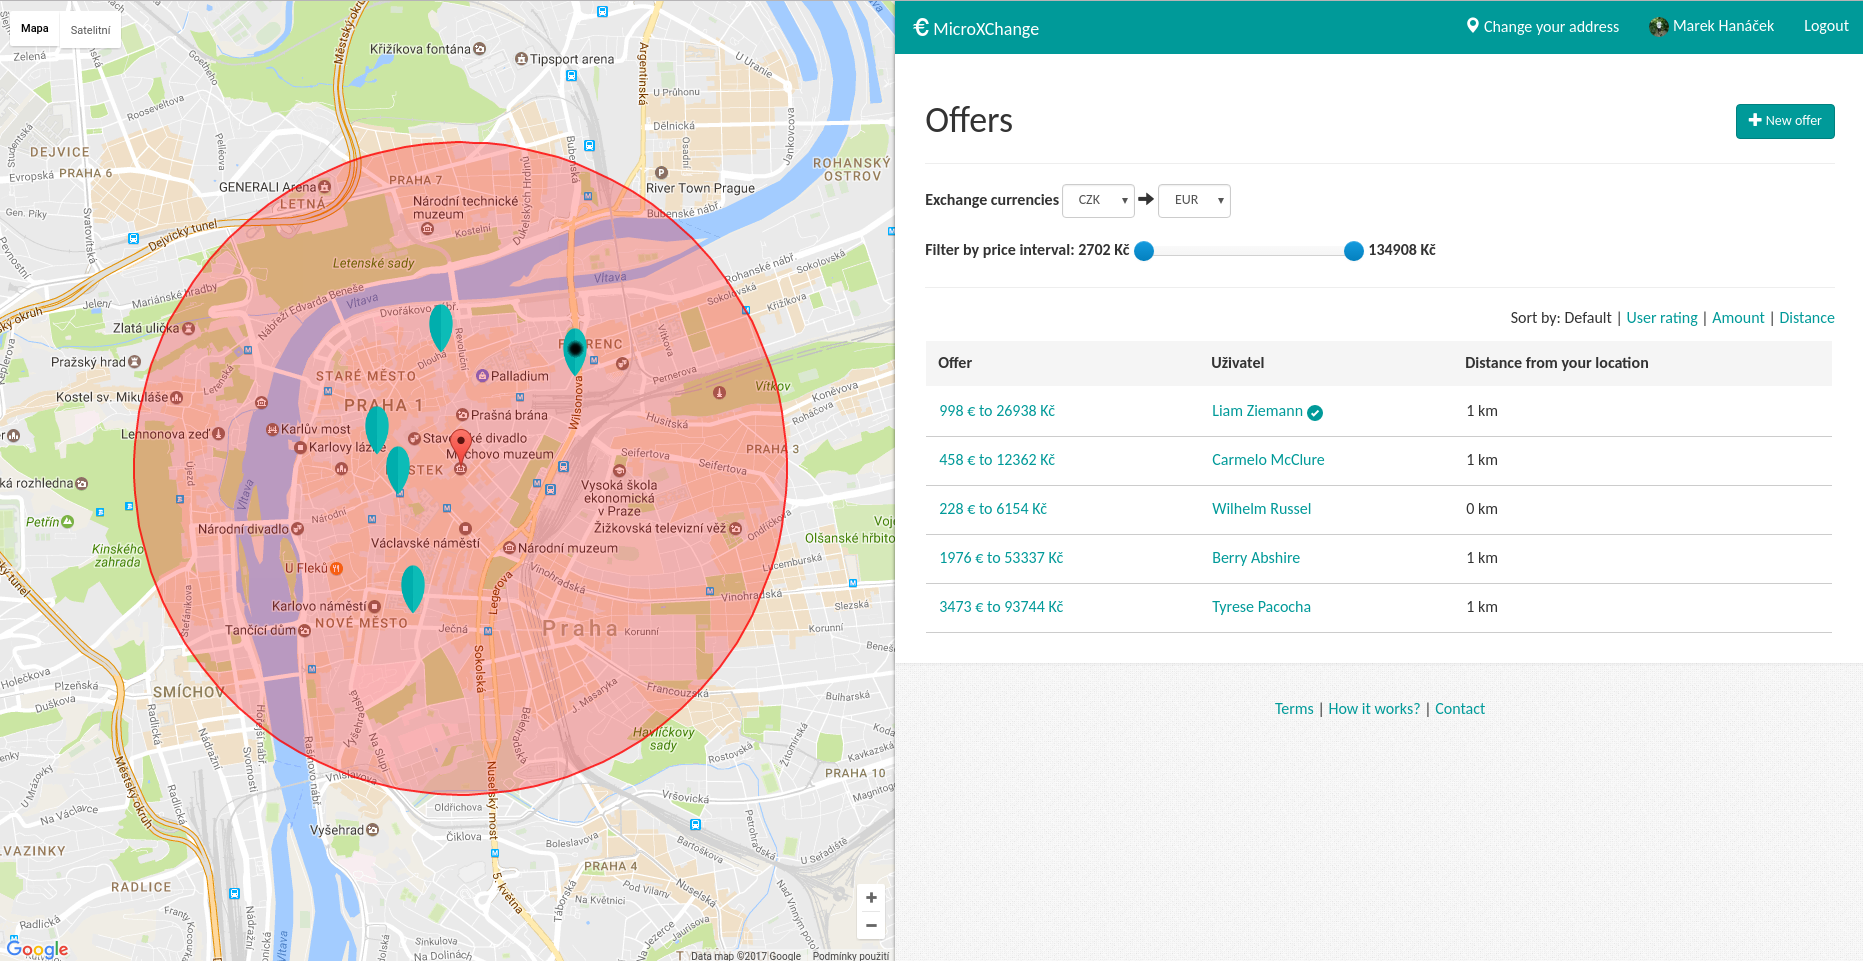
\includegraphics[width=1.0\textwidth]{media/tur/homepage.png}
    \caption{Hlavní stránka aplikace}
    \label{fig:tur:homepage}
\end{figure}

\subsection{Mapa}
Mapa obsahuje ukazatel polohy uživatele, kruh znázorňující vyhledávací poloměr a ukazatele poloh nabídek. Ukazatel polohy uživatele a poloh nabídek jsou barevně odlišeny.

\subsection{Textová část}
Textová část se skládá z~hlavičky, filtračního formuláře, seznamu nabídek s~možností seřazení, tlačítka pro vytvoření nové nabídky a patičky obsahující odkazy na informační stránky.

\subsection{Filtrace nabídek}
Formulář obsahuje tři základní parametry, pomocí nichž lze filtrovat:
\begin{itemize}
	\item Měnu, ze které chceme peníze směnit,
	\item měnu, do které chceme peníze směnit,
	\item interval obnosu peněz.
\end{itemize}
Filtrace dále bere v~potaz i aktuální polohu (respektive uživatelem zadanou polohu) a poloměr. Filtrace se samozřejmě projevuje i v~mapě. Jsou tedy zobrazeny jen ty nabídky, které odpovídají zadaným filtrům.

\subsection{Řazení nabídek}
Vidno na obrázku \ref{fig:tur:sorting}. Nabídky lze seřadit čtyřmi různými způsoby:
\begin{itemize}
	\item Vzestupně dle vzdálenosti polohy uživatele od centra nabídky.
	\item Vzestupně dle obnosu peněz nabídek.
	\item Sestupně dle hodnocení uživatelů.
	\item Dle kombinace více kritérií nabídek. Tento způsob blíže popisuji v~následující podkapitole.
\end{itemize}

\begin{figure}[!h]
    \centering
    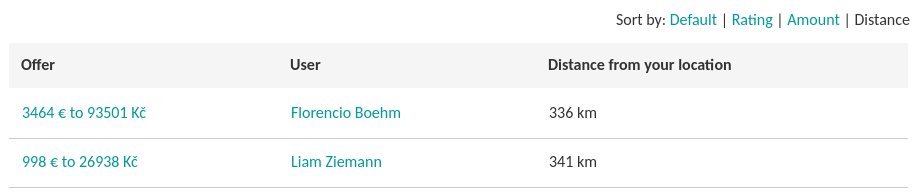
\includegraphics[width=1.0\textwidth]{media/tur/sorting.png}
    \caption{Výpis nabídek s~možností seřazení}
    \label{fig:tur:sorting}
\end{figure}

\subsubsection{Řazení nabídek dle kombinace více kritérií}
Hodnocení se skládá ze dvou složek:
\begin{itemize}
	\item Hodnocení uživatele:
        \begin{itemize}
            \item Jestliže má uživatel měně než dvě hodnocení, pak je tato hodnota rovna 0.
            \item Jestliže má uživatel dvě a více hodnocení, pak se hodnota odvíjí od průměrného počtu hvězdiček. Za špatné hodnocení je penalizován, za dobré hodnocení pak odměněn kladnými body. Konkrétně\footnote{Uvedené hodnocení a penalizace jsou založeny na základě experimentálního zkoumání řazení s~velkým množstvím testovacích dat.}:
            \begin{itemize}
                \item 1 hvězdička $\rightarrow$ penalizace $-1.5$,
                \item 2 hvězdičky $\rightarrow$ penalizace $-1$,
                \item 3 hvězdičky $\rightarrow$ hodnocení je rovno 0.6,
                \item 4 hvězdičky $\rightarrow$ hodnocení je rovno 0.8,
                \item 5 hvězdiček $\rightarrow$ hodnocení je rovno 1.
            \end{itemize}
        \end{itemize}
	\item Vzdálenost od uživatele:
        \begin{itemize}
            \item Za vzdálenost od uživatele může nabídka dostat 0 až 1 bod.
            \item Hodnota se počítá na základě vzdálenosti nejbližší a nejvzdálenější nabídky a dále na základě vzdálenosti právě hodnocené nabídky.
            \item Kód výpočtu této hodnoty lze vidět v~ukázce kódu \ref{code:sorting-distance}.
            \item Čím blíže je tedy nabídka k~zákazníkovi, tím lepší hodnocení obdrží.
            \item \textit{Příklad}: V~případě tři nabídek ve vzdálenostech 15~km, 2~km a 28~km, budou hodnocení 0.5, 1 a 0.
        \end{itemize}
\end{itemize}

\begin{listing}[htbp]
\caption{\label{code:sorting-distance}Funkce pro výpočet hodnocení vzdálenosti od uživatele}
\begin{minted}[frame=lines,bgcolor=codebg,fontsize=\footnotesize,linenos,breaklines]{Python}
def get_distance_rating(offer, min_distance, max_distance, lat, lng):
    """
    Keyword arguments:
    offer -- concrete offer
    min_distance -- distance of nearest offer
    max_distance -- distance of the furthest offer
    lat -- input latitude
    lng -- input longitude
    """
    distance_from_min = get_offer_distance_from(offer, lat, lng) - min_distance
    min_max_distance = max_distance - min_distance
    percent = min_max_distance / 100
    return 1 - ((distance_from_min / percent) / 100)
\end{minted}
\end{listing}

\subsection{Mobilní verze}
Stejně jako při návrhu desktopové verze, tak i při návrhu mobilní verze je návrh inspirován webem Sreality.cz, který byl analyzován v~kapitole \ref{analyza:sreality}. Zobrazuje se tedy vždy pouze mapa nebo textová část. Viz obrázek \ref{fig:tur:homepage-mobile} na straně \pageref{fig:tur:homepage-mobile}.

\begin{figure}[!h]
    \centering
    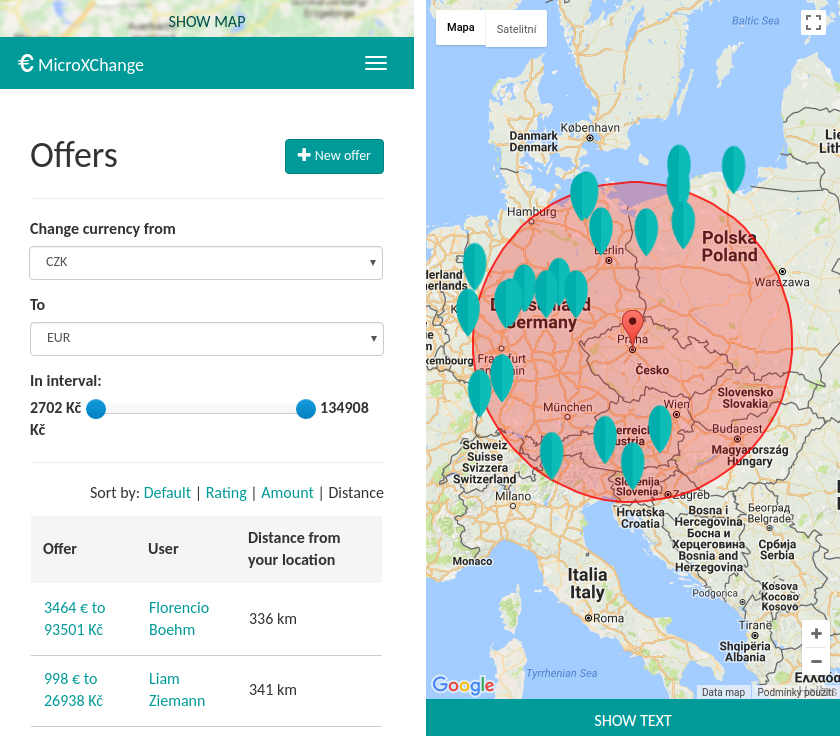
\includegraphics[width=1.0\textwidth]{media/tur/homepage-mobile.png}
    \caption{Mobilní verze aplikace}
    \label{fig:tur:homepage-mobile}
\end{figure}
